\chapter{Introduction}
\label{chp:intro}


%%%%%%%%%%%%%%%%%%%%%%%%%%%%%%%%%%%%%%%%%%%%%%%%%%%%%%%%%%%%%%%%%%%%%%%
\section{Background}
\label{sec:bg}
Unmanned Aerial Vehicles (UAVs) are a technology that have gained popularity in various applications recently\cite{CPP-Survey-2019}. Originally, UAVs required a ground pilot to manoeuvre them, but are becoming an increasingly automated technology. Applications where UAV automation has been used include, but are not limited to, structure inspections\cite{Guerrero2013}, smart farming\cite{Lottes2017}, disaster management\cite{Maza2011}, power line inspections\cite{Chang2017}, surveillance\cite{Basilico2015} and wildfire tracking\cite{Pham2017}.

Most of the research mentioned was done on the premise of using multi-rotor UAVs, quad-rotor vehicles in particular. It is important to note that the term UAVs also encompasses other aircraft types, like single rotor and fixed wing UAVs. Hybrids also exist that contain both rotary-wing and fixed-wing components\cite{CPP-Survey-2019}.

Using UAVs poses a considerable advantage in applications like the ones mentioned when compared to unmanned ground vehicles (UGVs). Their capacity to fly over landscapes and around three dimensional structures makes their potential applications increase substantially. Relatively high altitude flying is a key reason why they are well suited to the application suggested in this paper, which is coverage path planning for search and rescue missions.

Coverage path planning (CPP) is a variant of the general motion planning problem. Originally, motion planning algorithms were predominantly used to find solutions for start-goal problems\cite{Choset2001}. This implies finding a sequence of actions to get an object from some starting state to some goal state. An example would be finding a sequence of movements to get a robotic arm from one orientation to another. In the context of path planning it means getting an agent, a UAV for example, from some starting position to some goal position in an environment\cite{Lynch2017}.

Coverage path planning is different from start-goal path planning in that it tries to determine a path for an agent to pass over all points in an environment\cite{Choset2001}. It can be used with ground vehicles, for example, to automate field machines for smart farming\cite{Hameed2014}. Further examples include vacuum cleaning robots, spray painting robots\cite{Atkar2005}, window cleaning robots\cite{Mir-Nasiri2018} and automated lawn mowers\cite{Arkin1999}. For underwater vehicles it can be used for the inspection of difficult to reach underwater structures\cite{Englot2012}. 

Furthermore, there have been developments in the use of UAVs to perform automated search and rescue operations using coverage path planning. Perhaps the most notable example is a project by DroneSAR where they use DJI drones to perform search and rescue tasks. Their implementation includes a mobile application that allows the user to designate a search area manually\cite{DroneSAR01}. Search and rescue operations often span large areas and UAVs fly above most ground obstacles. Therefore, it is realistic to assume the environment can be mapped prior to the search operation\cite{CPP-Survey-2013}.

DroneSAR uses one drone per search and rescue operation. Once the environment has been designated, the drone performs a back and forth manoeuvre across the area to achieve coverage. The search operation can be halted if the imaging system detects a possible target in the area. The drone can be switched to manual flight mode for closer inspection and the co-ordinates of the target, for example a person in turmoil, can be sent to the search and rescue team. Their system also allows for the manual assignment of way-points to a flight path to bypass the back and forth manoeuvre.\cite{DroneSAR02}

In figure~\ref{fig:DroneSAR}, a screenshot of their mobile application is shown. It illustrates the back and forth manoeuvre used to achieve coverage of the designated area.

\begin{figure}[h]
	\centering
	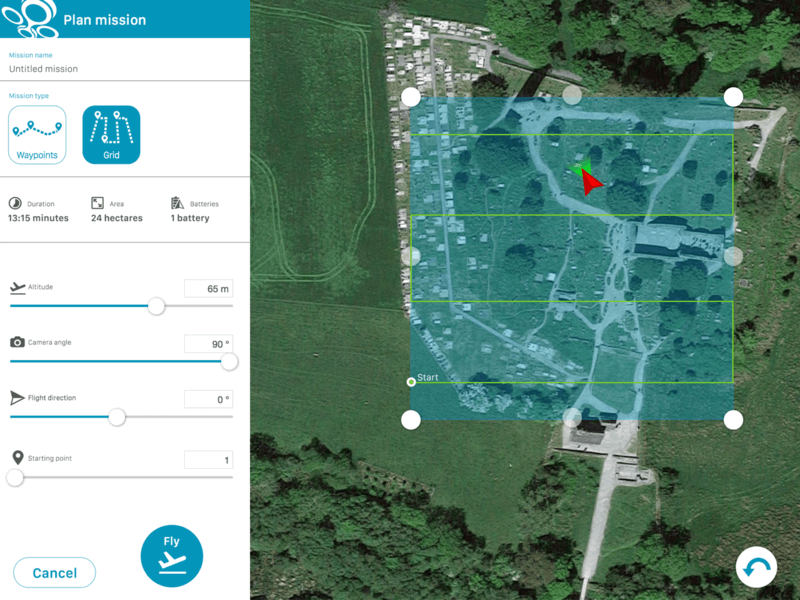
\includegraphics[scale=0.3]{figs/content_DroneSAR_screenshot_3.png}
	\caption{DroneSAR Mobile Application Showing Coverage Plan\cite{DroneSAR01}}
	\label{fig:DroneSAR}
\end{figure}

This paper also looks at coverage path planning for search and rescue, but suggests a multiple UAV approach to the problem. According to \cite{DroneSAR01}, when looking for a victim in a one square kilometre area on land, it takes a five-person rescue team two hours on average to find the victim. DroneSAR found that their drone could do the same job in under 20 minutes.
Adding multiple UAVs to cover an area could reduce this time even more, since it would mean more area is covered per unit time. This is important because in a search and rescue operation, time is always of the essence.

This paper also focuses on a grid-based approach to the coverage problem. According to the taxonomy represented in \cite{Choset2001}, this is referred to as an approximate method. Although one can achieve complete coverage of the grid, the grid itself is not an exact representation of the environment. It does, however, greatly simplify the process of allocating areas to different UAVs, which is a key process for multiple UAV coverage. Physical implementation of this method will not be addressed as part of the scope for this paper.

\section{Research Aim}
\label{sec:researchAim}
The main goal of this research is to develop a coverage path planning algorithm for multiple unmanned aerial vehicles (UAVs) to search an area. The research is intended to be applicable in search and rescue operations using unmanned aerial vehicles to assist.

\section{Research Objectives}
Based on the main aim of this project set out in section \ref{sec:researchAim}, a set of research objectives were formulated. These are intended to give a clearer picture of the main research goals and scope of the project. Scope and limitations are further discussed in section \ref{sec:scope} and the methodology used to achieve these objectives are detailed in section \ref{sec:method}. The research objectives are as follows:
\begin{enumerate}
	\item Develop a coverage path planning algorithm for an environment that is known a priori and contains static obstacles.
	\item Ensure that the final algorithm is an approximately complete solution.
	\item Incorporate into the algorithm's functionality an ability to have a changing number of starting UAVs that have random initial positions.
	\item Evaluate the algorithm's performance in both randomly generated and mapped, real world environments to ascertain whether or not it is suitable for search and rescue operations.
\end{enumerate}

\section{Scope and Limitations}
\label{sec:scope}

\section{Methodology}
\label{sec:method}

\section{Thesis Structure}
% Later